\documentclass[border=6pt]{standalone}
\usepackage{tikz}
\usetikzlibrary{arrows.meta,positioning,calc}
\begin{document}
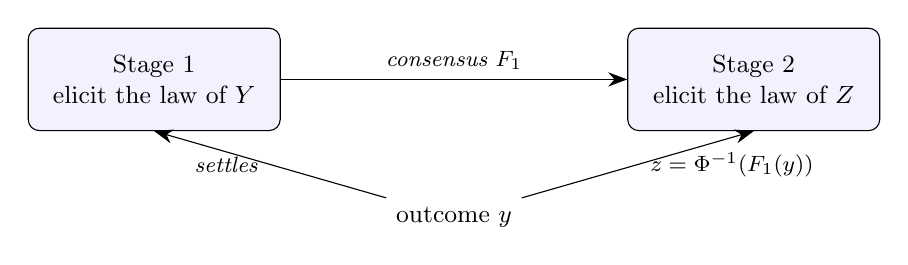
\begin{tikzpicture}[
  font=\small,
  box/.style={draw,rounded corners,minimum width=32mm,minimum height=13mm,
              align=center,fill=blue!5},
  lbl/.style={font=\footnotesize\itshape},
  >={Stealth[length=2.4mm]},
]
  \node[box] (s1) {Stage 1\\ elicit the law of $Y$};
  \node[box, right=44mm of s1] (s2) {Stage 2\\ elicit the law of $Z$};
  \node[below=15mm of $(s1)!0.5!(s2)$] (y) {outcome $y$};

  \draw[->] (s1) -- node[above,lbl] {consensus $F_1$} (s2);
  \draw[->] (y) -- node[left=1pt,lbl] {settles} (s1.south);
  \draw[->] (y) -- node[right=1pt,lbl] {$z=\Phi^{-1}(F_1(y))$} (s2.south);
\end{tikzpicture}
\end{document}
